
%% bare_conf.tex
%% V1.4b
%% 2015/08/26
%% by Michael Shell
%% See:
%% http://www.michaelshell.org/
%% for current contact information.
%%
%% This is a skeleton file demonstrating the use of IEEEtran.cls
%% (requires IEEEtran.cls version 1.8b or later) with an IEEE5
%% conference paper.
%%
%% Support sites:
%% http://www.michaelshell.org/tex/ieeetran/
%% http://www.ctan.org/pkg/ieeetran
%% and
%% http://www.ieee.org/

%%*************************************************************************
%% Legal Notice:
%% This code is offered as-is without any warranty either expressed or
%% implied; without even the implied warranty of MERCHANTABILITY or
%% FITNESS FOR A PARTICULAR PURPOSE! 
%% User assumes all risk.
%% In no event shall the IEEE or any contributor to this code be liable for
%% any damages or losses, including, but not limited to, incidental,
%% consequential, or any other damages, resulting from the use or misuse
%% of any information contained here.
%%
%% All comments are the opinions of their respective authors and are not
%% necessarily endorsed by the IEEE.
%%
%% This work is distributed under the LaTeX Project Public License (LPPL)
%% ( http://www.latex-project.org/ ) version 1.3, and may be freely used,
%% distributed and modified. A copy of the LPPL, version 1.3, is included
%% in the base LaTeX documentation of all distributions of LaTeX released
%% 2003/12/01 or later.
%% Retain all contribution notices and credits.
%% ** Modified files should be clearly indicated as such, including  **
%% ** renaming them and changing author support contact information. **
%%*************************************************************************


% *** Authors should verify (and, if needed, correct) their LaTeX system  ***
% *** with the testflow diagnostic prior to trusting their LaTeX platform ***
% *** with production work. The IEEE's font choices and paper sizes can   ***
% *** trigger bugs that do not appear when using other class files.       ***                          ***
% The testflow support page is at:
% http://www.michaelshell.org/tex/testflow/



\documentclass[conference]{IEEEtran}
% Some Computer Society conferences also require the compsoc mode option,
% but others use the standard conference format.
%
% If IEEEtran.cls has not been installed into the LaTeX system files,
% manually specify the path to it like:
% \documentclass[conference]{../sty/IEEEtran}


% *** STUFF WE ADD THAT THE PACKAGE SHOULD HAVE HAD ***




%Math Packages
\usepackage{amsmath}
\usepackage{amsfonts}
\usepackage{amssymb}
\usepackage{kbordermatrix}
\renewcommand{\kbldelim}{[}% Left delimiter
\renewcommand{\kbrdelim}{]}% Right delimiter
\usepackage{siunitx}

\usepackage{bbm}
%-----------------------------------------%
\usepackage{hyperref}
\usepackage{amsthm}
\usepackage[capitalise]{cleveref}

\usepackage[]{graphicx}
\usepackage{tikz}
\usetikzlibrary{shapes,shapes.geometric, arrows,positioning,calc}
\tikzset{
	block/.style = {draw, fill=white, rectangle, minimum height=3em, minimum width=3em},
	tmp/.style  = {coordinate}, 
	sum/.style= {draw, fill=white, circle, node distance=1cm},
	input/.style = {coordinate},
	output/.style= {coordinate},
	pinstyle/.style = {pin edge={to-,thin,black}
	}
}

% Setup for use of lemmas and theorems

\newtheorem{thm}{Theorem}
\newtheorem{lem}[thm]{Lemma}
\newtheorem{cor}[thm]{Corollary}
\newtheorem{rem}[thm]{Remark}
\newtheorem{remark}[thm]{Remark}
\newtheorem{conj}[thm]{Conjecture}

% Table stuff
\usepackage{booktabs}

% Some very useful LaTeX packages include:
% (uncomment the ones you want to load)


% *** MISC UTILITY PACKAGES ***
%
%\usepackage{ifpdf}
% Heiko Oberdiek's ifpdf.sty is very useful if you need conditional
% compilation based on whether the output is pdf or dvi.
% usage:
% \ifpdf
%   % pdf code
% \else
%   % dvi code
% \fi
% The latest version of ifpdf.sty can be obtained from:
% http://www.ctan.org/pkg/ifpdf
% Also, note that IEEEtran.cls V1.7 and later provides a builtin
% \ifCLASSINFOpdf conditional that works the same way.
% When switching from latex to pdflatex and vice-versa, the compiler may
% have to be run twice to clear warning/error messages.


% *** CITATION PACKAGES ***
%
%\usepackage{cite}
% cite.sty was written by Donald Arseneau
% V1.6 and later of IEEEtran pre-defines the format of the cite.sty package
% \cite{} output to follow that of the IEEE. Loading the cite package will
% result in citation numbers being automatically sorted and properly
% "compressed/ranged". e.g., [1], [9], [2], [7], [5], [6] without using
% cite.sty will become [1], [2], [5]--[7], [9] using cite.sty. cite.sty's
% \cite will automatically add leading space, if needed. Use cite.sty's
% noadjust option (cite.sty V3.8 and later) if you want to turn this off
% such as if a citation ever needs to be enclosed in parenthesis.
% cite.sty is already installed on most LaTeX systems. Be sure and use
% version 5.0 (2009-03-20) and later if using hyperref.sty.
% The latest version can be obtained at:
% http://www.ctan.org/pkg/cite
% The documentation is contained in the cite.sty file itself.






% *** GRAPHICS RELATED PACKAGES ***
%
\ifCLASSINFOpdf
  % \usepackage[pdftex]{graphicx}
  % declare the path(s) where your graphic files are
  % \graphicspath{{../pdf/}{../jpeg/}}
  % and their extensions so you won't have to specify these with
  % every instance of \includegraphics
  % \DeclareGraphicsExtensions{.pdf,.jpeg,.png}
\else
  % or other class option (dvipsone, dvipdf, if not using dvips). graphicx
  % will default to the driver specified in the system graphics.cfg if no
  % driver is specified.
  % \usepackage[dvips]{graphicx}
  % declare the path(s) where your graphic files are
  % \graphicspath{{../eps/}}
  % and their extensions so you won't have to specify these with
  % every instance of \includegraphics
  % \DeclareGraphicsExtensions{.eps}
\fi
% graphicx was written by David Carlisle and Sebastian Rahtz. It is
% required if you want graphics, photos, etc. graphicx.sty is already
% installed on most LaTeX systems. The latest version and documentation
% can be obtained at: 
% http://www.ctan.org/pkg/graphicx
% Another good source of documentation is "Using Imported Graphics in
% LaTeX2e" by Keith Reckdahl which can be found at:
% http://www.ctan.org/pkg/epslatex
%
% latex, and pdflatex in dvi mode, support graphics in encapsulated
% postscript (.eps) format. pdflatex in pdf mode supports graphics
% in .pdf, .jpeg, .png and .mps (metapost) formats. Users should ensure
% that all non-photo figures use a vector format (.eps, .pdf, .mps) and
% not a bitmapped formats (.jpeg, .png). The IEEE frowns on bitmapped formats
% which can result in "jaggedy"/blurry rendering of lines and letters as
% well as large increases in file sizes.
%
% You can find documentation about the pdfTeX application at:
% http://www.tug.org/applications/pdftex





% *** MATH PACKAGES ***
%
%\usepackage{amsmath}
% A popular package from the American Mathematical Society that provides
% many useful and powerful commands for dealing with mathematics.
%
% Note that the amsmath package sets \interdisplaylinepenalty to 10000
% thus preventing page breaks from occurring within multiline equations. Use:
%\interdisplaylinepenalty=2500
% after loading amsmath to restore such page breaks as IEEEtran.cls normally
% does. amsmath.sty is already installed on most LaTeX systems. The latest
% version and documentation can be obtained at:
% http://www.ctan.org/pkg/amsmath





% *** SPECIALIZED LIST PACKAGES ***
%
%\usepackage{algorithmic}
% algorithmic.sty was written by Peter Williams and Rogerio Brito.
% This package provides an algorithmic environment fo describing algorithms.
% You can use the algorithmic environment in-text or within a figure
% environment to provide for a floating algorithm. Do NOT use the algorithm
% floating environment provided by algorithm.sty (by the same authors) or
% algorithm2e.sty (by Christophe Fiorio) as the IEEE does not use dedicated
% algorithm float types and packages that provide these will not provide
% correct IEEE style captions. The latest version and documentation of
% algorithmic.sty can be obtained at:
% http://www.ctan.org/pkg/algorithms
% Also of interest may be the (relatively newer and more customizable)
% algorithmicx.sty package by Szasz Janos:
% http://www.ctan.org/pkg/algorithmicx




% *** ALIGNMENT PACKAGES ***
%
%\usepackage{array}
% Frank Mittelbach's and David Carlisle's array.sty patches and improves
% the standard LaTeX2e array and tabular environments to provide better
% appearance and additional user controls. As the default LaTeX2e table
% generation code is lacking to the point of almost being broken with
% respect to the quality of the end results, all users are strongly
% advised to use an enhanced (at the very least that provided by array.sty)
% set of table tools. array.sty is already installed on most systems. The
% latest version and documentation can be obtained at:
% http://www.ctan.org/pkg/array


% IEEEtran contains the IEEEeqnarray family of commands that can be used to
% generate multiline equations as well as matrices, tables, etc., of high
% quality.




% *** SUBFIGURE PACKAGES ***
\ifCLASSOPTIONcompsoc
  \usepackage[caption=false,font=normalsize,labelfont=sf,textfont=sf]{subfig}
\else
  \usepackage[caption=false,font=footnotesize]{subfig}
\fi
% subfig.sty, written by Steven Douglas Cochran, is the modern replacement
% for subfigure.sty, the latter of which is no longer maintained and is
% incompatible with some LaTeX packages including fixltx2e. However,
% subfig.sty requires and automatically loads Axel Sommerfeldt's caption.sty
% which will override IEEEtran.cls' handling of captions and this will result
% in non-IEEE style figure/table captions. To prevent this problem, be sure
% and invoke subfig.sty's "caption=false" package option (available since
% subfig.sty version 1.3, 2005/06/28) as this is will preserve IEEEtran.cls
% handling of captions.
% Note that the Computer Society format requires a larger sans serif font
% than the serif footnote size font used in traditional IEEE formatting
% and thus the need to invoke different subfig.sty package options depending
% on whether compsoc mode has been enabled.
%
% The latest version and documentation of subfig.sty can be obtained at:
% http://www.ctan.org/pkg/subfig




% *** FLOAT PACKAGES ***
%
%\usepackage{fixltx2e}
% fixltx2e, the successor to the earlier fix2col.sty, was written by
% Frank Mittelbach and David Carlisle. This package corrects a few problems
% in the LaTeX2e kernel, the most notable of which is that in current
% LaTeX2e releases, the ordering of single and double column floats is not
% guaranteed to be preserved. Thus, an unpatched LaTeX2e can allow a
% single column figure to be placed prior to an earlier double column
% figure.
% Be aware that LaTeX2e kernels dated 2015 and later have fixltx2e.sty's
% corrections already built into the system in which case a warning will
% be issued if an attempt is made to load fixltx2e.sty as it is no longer
% needed.
% The latest version and documentation can be found at:
% http://www.ctan.org/pkg/fixltx2e


%\usepackage{stfloats}
% stfloats.sty was written by Sigitas Tolusis. This package gives LaTeX2e
% the ability to do double column floats at the bottom of the page as well
% as the top. (e.g., "\begin{figure*}[!b]" is not normally possible in
% LaTeX2e). It also provides a command:
%\fnbelowfloat
% to enable the placement of footnotes below bottom floats (the standard
% LaTeX2e kernel puts them above bottom floats). This is an invasive package
% which rewrites many portions of the LaTeX2e float routines. It may not work
% with other packages that modify the LaTeX2e float routines. The latest
% version and documentation can be obtained at:
% http://www.ctan.org/pkg/stfloats
% Do not use the stfloats baselinefloat ability as the IEEE does not allow
% \baselineskip to stretch. Authors submitting work to the IEEE should note
% that the IEEE rarely uses double column equations and that authors should try
% to avoid such use. Do not be tempted to use the cuted.sty or midfloat.sty
% packages (also by Sigitas Tolusis) as the IEEE does not format its papers in
% such ways.
% Do not attempt to use stfloats with fixltx2e as they are incompatible.
% Instead, use Morten Hogholm'a dblfloatfix which combines the features
% of both fixltx2e and stfloats:
%
% \usepackage{dblfloatfix}
% The latest version can be found at:
% http://www.ctan.org/pkg/dblfloatfix




% *** PDF, URL AND HYPERLINK PACKAGES ***
%
%\usepackage{url}
% url.sty was written by Donald Arseneau. It provides better support for
% handling and breaking URLs. url.sty is already installed on most LaTeX
% systems. The latest version and documentation can be obtained at:
% http://www.ctan.org/pkg/url
% Basically, \url{my_url_here}.




% *** Do not adjust lengths that control margins, column widths, etc. ***
% *** Do not use packages that alter fonts (such as pslatex).         ***
% There should be no need to do such things with IEEEtran.cls V1.6 and later.
% (Unless specifically asked to do so by the journal or conference you plan
% to submit to, of course. )


% correct bad hyphenation here
\hyphenation{op-tical net-works semi-conduc-tor}


\begin{document}
%
% paper title
% Titles are generally capitalized except for words such as a, an, and, as,
% at, but, by, for, in, nor, of, on, or, the, to and up, which are usually
% not capitalized unless they are the first or last word of the title.
% Linebreaks \\ can be used within to get better formatting as desired.
% Do not put math or special symbols in the title.
\title{Modelling and Networked Control of Water Distribution Networks}


% author names and affiliations
% use a multiple column layout for up to three different
% affiliations
%\author{\IEEEauthorblockN{Michael Shell}
%\IEEEauthorblockA{School of Electrical and\\Computer Engineering\\
%Georgia Institute of Technology\\
%Atlanta, Georgia 30332--0250\\
%Email: http://www.michaelshell.org/contact.html}
%\and
%\IEEEauthorblockN{Homer Simpson}
%\IEEEauthorblockA{Twentieth Century Fox\\
%Springfield, USA\\
%Email: homer@thesimpsons.com}
%\and
%\IEEEauthorblockN{James Kirk\\ and Montgomery Scott}
%\IEEEauthorblockA{Starfleet Academy\\
%	San Francisco, California 96678--2391\\
%	Telephone: (800) 555--1212\\
%	Fax: (888) 555--1212}}

% conference papers do not typically use \thanks and this command
% is locked out in conference mode. If really needed, such as for
% the acknowledgment of grants, issue a \IEEEoverridecommandlockouts
% after \documentclass

% for over three affiliations, or if they all won't fit within the width
% of the page, use this alternative format:
% 
\author{\IEEEauthorblockN{
Martin Højlund Therkildsen\IEEEauthorrefmark{0},
Rasmus Løvschall Kristiansen\IEEEauthorrefmark{0},
Kasper Laustsen\IEEEauthorrefmark{0}, 
Jeppe Nørgaard Jensen\IEEEauthorrefmark{0},\\
Laurits Hastrup Andersen\IEEEauthorrefmark{0},
Mathias Clement Frederiksen\IEEEauthorrefmark{0} and 
Christian Møller Jensen\IEEEauthorrefmark{0}}
\\ 
\IEEEauthorblockA{\IEEEauthorrefmark{0}Technical Faculty of IT and Design, Department of Electronic Systems, Aalborg University
\\ Email: es-21-ca-7-733@student.aau.dk}
}



% use for special paper notices
%\IEEEspecialpapernotice{(Invited Paper)}




% make the title area
\maketitle

% As a general rule, do not put math, special symbols or citations
% in the abstract
\begin{abstract}\label{sec:Abstract}
High quality control of Water Distribution Networks (WDN) is critical to reliable supply of drinking water to consumers, but is subject to complex nonlinear dynamics and delays induced by actuator characteristics and long-distance wireless communication. This paper proposes a cascaded control system that delivers a constant elevated reservoir level via an outer velocity-form Linear Quadratic Regulator (VF-LQR) and an inner PID pump control loop. Furthermore, disturbance rejection in the outer loop and leakage detection are facilitated by a Kalman filter (KF). The paper presents comprehensive simulation and experimental validation of the proposed control design, as well as a worst-case analysis of robustness under feedback delay induced by wireless communication losses.
\end{abstract}

% no keywords




% For peer review papers, you can put extra information on the cover
% page as needed:
% \ifCLASSOPTIONpeerreview
% \begin{center} \bfseries EDICS Category: 3-BBND \end{center}
% \fi
%
% For peerreview papers, this IEEEtran command inserts a page break and
% creates the second title. It will be ignored for other modes.
\IEEEpeerreviewmaketitle


\section{Introduction}\label{sec:Introduction}
%This article is the main product of the $7$th-semester project on the MSc degree in Control and Automation at Aalborg university. The project focuses on the subject of Water Distributed Networks (WDN), specifically modelling and control of these. Control strategies used include Linear–quadratic regulator (LQR) and Proportional Integral controller (PI). Further more Kalmann filter is used to estimate shit.... The project also investigates packet-loss in the feedback loop to the LQR. 

Water Distribution Networks (WDN) are a key infrastructure element that facilitates the supply of drinking water from a water source to end users. They consist of pumping stations, consumers, a network of pipes, and typically one or more elevated water reservoirs (EWR) \cite{Swamee2008}. The latter in particular play an important role in pressure regulation, peak demand matching, and backup supply in case of e.g. pump failure \cite{Creaco2019}. Furthermore, they allow for energy-efficient pump scheduling \cite{Rathore1030,Bello2019}.  

Failure to manage tank level appropriately relative to consumer demand may lead to system overpressure and an accompanying risk of pipe damage and water leakage when demand is low, or to system underpressure and insufficient service pressure provided to consumers when demand is high. Optimisation-based control schemes such as Model-Predictive-Control are common \cite{OcampoMartinez2013,Kallesoe2017}, with data-driven plug-and-play approaches appearing in recent years \cite{Val2020}, particularly for large-scale systems.  

This paper presents a cascaded optimal control paradigm that exploits the separability of WDN dynamics into a slow tank pressure regime and a fast flow regime. The slow dynamics are paired with a velocity-form Linear Quadratic Regulator (VF-LQR) as seen in e.g. \cite{Pannocchia2015a}, while the fast dynamics are paired with PID regulators. Rejection of unmeasured time-varying disturbances and leakage detection is achieved using a Kalman filter based on a harmonic model, improving on e.g. \cite{OcampoMartinez2013} and \cite{Val2020} which respectively assume measurable or constant disturbances.

The remainder of this paper is organised as follows: in \Cref{sec:SysModel} we develop models of the fast and slow regimes of the system, including a linearised model of the fast regime. \Cref{sec:ControlStructure} details the structure and design of the VF-LQR and PID controllers as well as the disturbance rejection. \Cref{sec:Results} presents simulation and experimental results, as well as an overview of the laboratory testbed. Finally, \Cref{sec:Conclusion} summarises the contributions made in the paper, as well as ideas pertaining to future work.


% An example of a floating figure using the graphicx package.
% Note that \label must occur AFTER (or within) \caption.
% For figures, \caption should occur after the \includegraphics.
% Note that IEEEtran v1.7 and later has special internal code that
% is designed to preserve the operation of \label within \caption
% even when the captionsoff option is in effect. However, because
% of issues like this, it may be the safest practice to put all your
% \label just after \caption rather than within \caption{}.
%
% Reminder: the "draftcls" or "draftclsnofoot", not "draft", class
% option should be used if it is desired that the figures are to be
% displayed while in draft mode.
%
%\begin{figure}[!t]
%\centering
%\includegraphics[width=2.5in]{myfigure}
% where an .eps filename suffix will be assumed under latex, 
% and a .pdf suffix will be assumed for pdflatex; or what has been declared
% via \DeclareGraphicsExtensions.
%\caption{Simulation results for the network.}
%\label{fig_sim}
%\end{figure}

% Note that the IEEE typically puts floats only at the top, even when this
% results in a large percentage of a column being occupied by floats.


% An example of a double column floating figure using two subfigures.
% (The subfig.sty package must be loaded for this to work.)
% The subfigure \label commands are set within each subfloat command,
% and the \label for the overall figure must come after \caption.
% \hfil is used as a separator to get equal spacing.
% Watch out that the combined width of all the subfigures on a 
% line do not exceed the text width or a line break will occur.
%
%\begin{figure*}[!t]
%\centering
%\subfloat[Case I]{\includegraphics[width=2.5in]{box}%
%\label{fig_first_case}}
%\hfil
%\subfloat[Case II]{\includegraphics[width=2.5in]{box}%
%\label{fig_second_case}}
%\caption{Simulation results for the network.}
%\label{fig_sim}
%\end{figure*}
%
% Note that often IEEE papers with subfigures do not employ subfigure
% captions (using the optional argument to \subfloat[]), but instead will
% reference/describe all of them (a), (b), etc., within the main caption.
% Be aware that for subfig.sty to generate the (a), (b), etc., subfigure
% labels, the optional argument to \subfloat must be present. If a
% subcaption is not desired, just leave its contents blank,
% e.g., \subfloat[].


% An example of a floating table. Note that, for IEEE style tables, the
% \caption command should come BEFORE the table and, given that table
% captions serve much like titles, are usually capitalized except for words
% such as a, an, and, as, at, but, by, for, in, nor, of, on, or, the, to
% and up, which are usually not capitalized unless they are the first or
% last word of the caption. Table text will default to \footnotesize as
% the IEEE normally uses this smaller font for tables.
% The \label must come after \caption as always.
%
%\begin{table}[!t]
%% increase table row spacing, adjust to taste
%\renewcommand{\arraystretch}{1.3}
% if using array.sty, it might be a good idea to tweak the value of
% \extrarowheight as needed to properly center the text within the cells
%\caption{An Example of a Table}
%\label{table_example}
%\centering
%% Some packages, such as MDW tools, offer better commands for making tables
%% than the plain LaTeX2e tabular which is used here.
%\begin{tabular}{|c||c|}
%\hline
%One & Two\\
%\hline
%Three & Four\\
%\hline
%\end{tabular}
%\end{table}


% Note that the IEEE does not put floats in the very first column
% - or typically anywhere on the first page for that matter. Also,
% in-text middle ("here") positioning is typically not used, but it
% is allowed and encouraged for Computer Society conferences (but
% not Computer Society journals). Most IEEE journals/conferences use
% top floats exclusively. 
% Note that, LaTeX2e, unlike IEEE journals/conferences, places
% footnotes above bottom floats. This can be corrected via the
% \fnbelowfloat command of the stfloats package.

\section{System Modelling}\label{sec:SysModel}
The WDN of concern in this paper is a two-pump, two-consumer, single-EWR system as seen on \cref{fig:WDNModel}.

\begin{figure}[h]
	\centering
	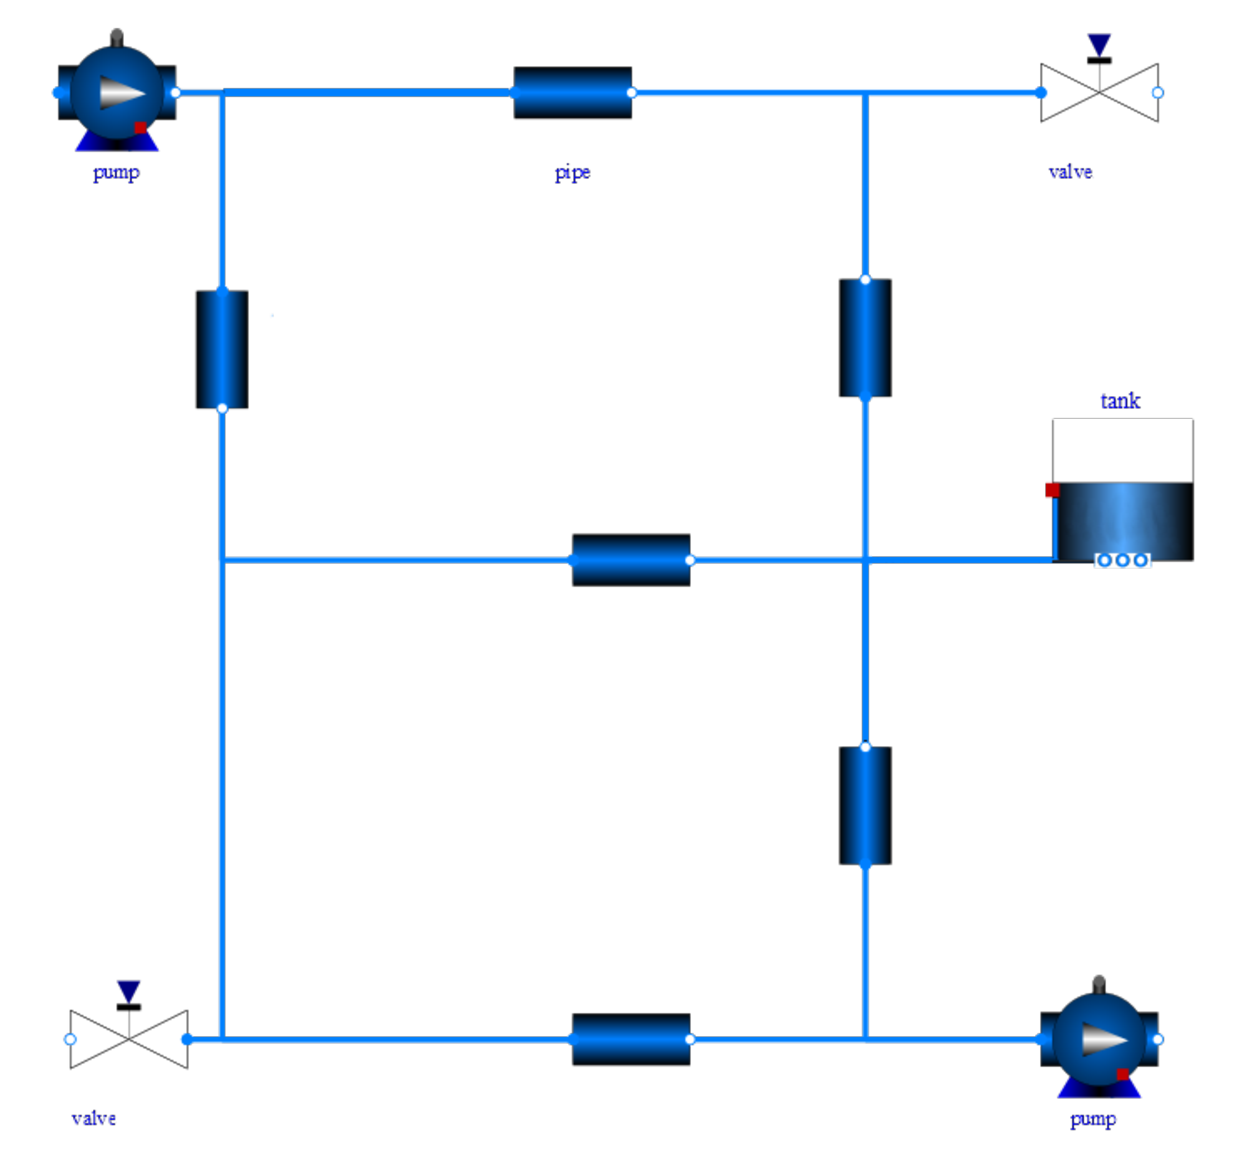
\includegraphics[width=0.5\linewidth]{Graphics/WDNModel.pdf}
	\caption{Schematic of the WDN under study.}
	\label{fig:WDNModel}
\end{figure}

As described in \Cref{sec:Introduction}, the dynamics of a WDN can be separated into a tank slow pressure regime and a fast flow regime. We use a directed graph model of the WDN corresponding to \cref{fig:tikzWDNGraph}, with the vertices $\{v_1,..,v_n\}$, edges $\{e_1,..,e_m\}$, nodal demands and nodal heights $d_i, h_i$ and edge flows $q_i$:

\begin{figure}[h!]
	\centering
	\resizebox{\columnwidth}{!}{
			\begin{tikzpicture}[node distance=30mm, thick, main/.style = {draw,circle}] 
		\node (1)  {};
		\node[main] (2) [node distance={15mm},right of=1] {$v_1$}; 
		\node[main] (3) [node distance={1.5cm},right of=2] {$v_2$};
		\node[main] (4) [right of=3] {$v_3$};
		\node[main] (5) [right of=4] {$v_4$};
		\node[main] (6) [right of=5] {$v_5$};
		\node (7) [node distance={15mm},right of=6] {};
		%Create 3 (4) nodes in middle part of graph
		\node[main] (8) [below of=4] {$ v_6 $};
		\node[main] (9) [node distance={20mm},below of=5] {$ v_7 $};
		\node[main] (11) [node distance={15mm},below of=9] {$ v_8 $};
		\node (10) [node distance={15mm},right of=11] {};
		%First 5 (7) nodes in bottom part of graph
		\node[main] (12) [below of=8] {$ v_{10} $};
		\node[main] (13) [left of=12] {$ v_9 $};
		\node(14) [node distance={15mm},left of=13] {};
		\node[main] (15) [right of=12] {$ v_{11} $};
		\node[main] (16) [right of=15] {$ v_{12} $};
		\node[main] (17) [node distance={1.5cm},right of=16] {$ v_{13} $};
		\node(18) [node distance={15mm},right of=17] {};
		
		%Edges with direction
		\path [->] (2) edge node[above] {$e_{1}$} (3); 	%Edge v1 -> v2
		\path [->] (3) edge node[above] {$e_{2}$} (4); 	%Edge v2 -> v3
		\path [->] (4) edge node[above] {$e_{3}$} (5); 	%Edge v3 -> v4
		\path [->] (5) edge node[above] {$e_{4}$} (6); 	%Edge v4 -> v5
		
		\path [->] (4) edge node[left] {$e_{5}$} (8); 	%Edge v3 -> v6
		\path [->] (5) edge node[right] {$e_{6}$} (9); 	%Edge v4 -> v7
		\path [->] (8) edge node[above] {$e_{7}$} (9); 	%Edge v6 -> v7
		\path [->] (8) edge node[left] {$e_{8}$} (12); 	%Edge v6 -> v10
		\path [->] (9) edge node[right] {$e_{9}$} (11); 	%Edge v7 -> v8
		\path [->] (11) edge node[right] {$e_{10}$} (15);	 %Edge v8 -> v11
		
		
		\path [->] (12) edge node[below] {$e_{11}$} (13); %Edge v10 -> v9
		\path [->] (15) edge node[below] {$e_{12}$} (12); %Edge v11 -> v10
		\path [->] (16) edge node[below] {$e_{13}$} (15); %Edge v12 -> v11
		\path [->] (17) edge node[below] {$e_{14}$} (16); %Edge v13 -> v12
		
		%External flows
		\draw[->,dashed,] (1) -- node[above] {$d_1$} (2); %Create d1
		\draw[->,dashed,] (6) -- node[above] {$d_5$} (7); %Create d5
		\draw[->,dashed,] (13) -- node[above] {$d_9$} (14); %Create d13
		\draw[->,dashed,] (18) -- node[above] {$d_{13}$} (17); %Create d13
		\draw[<->,dashed,] (10) -- node[above] {$d_\tau$} (11); %Create d_tau
	\end{tikzpicture} }
	\caption{Graph Network of Water Distributed Network. Note that $e_1$ and $e_{14} $ are only inserted to be able to measure pump flow}
	\label{fig:tikzWDNGraph}
\end{figure}  

Applying standard graph theory - see e.g. \cite{Deo} - to the graph, we obtain an incidence matrix $H$ and loop matrix $B$ with the chords $E_C=\{e_3,e_7\}$ chosen.

%\begin{equation*}
%	H_{i,j} = \begin{cases}
%		-1 & \text{If the $j^{th}$ edge enters the $i^{th}$ node} \\
%		0 & \text{If the $j^{th}$ edge is unconnected to the $i^{th}$ node} \\
%		1 & \text{If the $j^{th}$ edge leaves the $i^{th}$ node}
%	\end{cases}
%\end{equation*} %Description of the incident matrix
%
%\begin{equation*}
%	B_{i,j} = \begin{cases}
%		1 & \text{If the direction of the $ i^{th} $ loop and the} \\& \text{$j^{th}$ edge agree}\\
%		-1 & \text{If the direction of the $ i^{th} $ loop and the} \\& \text{$j^{th}$ edge do not agree}\\
%		0 & \text{If the $ i^{th} $ loop does not include the $ j^{th} $ edge}\\
%	\end{cases}
%\end{equation*}

We furthermore introduce the notation $H_T$ for the columns of $H$ in the spanning tree $E_T=\{e_1,e_2,e_4,..,e_6,e_8,..,e_{14}\}$, while $H_C$ is given by the columns of $H$ in $E_C=\{e_3,e_7\}$. The reduced incidence matrix $\bar{H}$ is obtained by choosing the node $ v_{13} $ as reference and eliminating the corresponding row of $H$.

In addition to these graph-related definitions, we require a few boundary conditions imposed by Kirchhoff's laws, which for an open WDN are given \cite{Jensen} by:
\begin{gather}
	Hq = d \label{eq:KirchNodeLaw} \\
	B\Delta p = B H^T p = 0 \wedge B\Delta h = B H^T h = 0 \label{eq:KirchMeshLaw}
\end{gather} 

Where $p$ is the vector of nodal pressures. Furthermore, mass conservation is assumed. This implies that there can at most be $n-1$ independent nodal demands, i.e.:

\begin{equation}\label{eq:MassConservation}
	d_n = -\sum_{i=1}^{n-1}d_i
\end{equation}

%Secondly, we require two lemmas pertaining to the spanning tree subspace $H_T$ of $H$: \\
%
%\begin{lem}\label{lem:TreePartitionLemma}
%	Let $H_T$ be the incidence matrix partition corresponding to the spanning tree of the graph described by $H$, and let $\bar{H}_T$ be its equivalent with respect to the reduced incidence matrix $\bar{H}$. $\bar{H}_T$ is invertible since a tree is a connected graph with $n-1$ edges \cite{Deo}, and the following holds:
%	
%	\begin{equation}\label{eq:TreePartitionLemma}
%		H_T\bar{H}_T^{-1} = \begin{bmatrix} I_{n-1} \\ \mathbbm{1}^T	\end{bmatrix}
%	\end{equation}
%	
%	where $\mathbbm{1}$ is a vector of ones and $I_{n-1} \in \mathbb{R}^{n-1 \times n-1}$ is an identity matrix.
%\end{lem}
%
%\newpage
%
%\begin{lem}\label{lem:EdgeFlowDecomposition}
%	Let $q \in \mathbb{R}^m$ be the edge flows of a graph with reduced incidence matrix $\bar{H}$ and $n$ nodes. Denote its spanning tree by $T$, let $q_c \in \mathbb{R}^c, \ c = m-n+1$ be the graph's chordal flows, and denote the tree partition of the reduced incidence matrix $\bar{H}_T$. Finally, let $B$ be the graph's fundamental loop matrix, and define $\bar{d} \in \mathbb{R}^{n-1}$ as the vector of non-reference nodal demands. Then the following is true:
%	
%	\begin{equation}\label{eq:EdgeFlowDecomposition}
%		q = B^T q_c +
%		\begin{bmatrix}
%			0_{c \times n-1} \\ \bar{H}_T^{-1} 
%		\end{bmatrix}
%		\bar{d}
%	\end{equation}
%\end{lem}
%
%With these definitions in hand, we move on to modelling of the slow dynamics.

\subsection{Slow Dynamics}\label{subsec:SlowDynamics}

The evolution of pressure $p_\tau$ in an EWR, assuming only one tank orifice, and defining the positive flow direction as \textit{from} the tank, can be described \cite{Jensen,Suresh2009} by the equation:

\begin{gather}\label{eq:TankPressureDyn}
	\dot{p}_\tau = -\tau d_\tau
	\\ \tau = \rho g \frac{1}{A_\tau}
\end{gather}

where $\rho$ is the density of the working fluid, $g$ is gravitational acceleration, and $A_\tau$ is the cross-sectional area of the tank. This can be discretised by Euler's method such that:

\begin{equation}\label{eq:DiscreteTankPressureDyn}
	p_\tau(k+1) = p_\tau(k) - \tau d_\tau(k)t_s =  p_\tau(k) - \mathcal{T} d_\tau(k)
\end{equation}

Now by the mass conservation condition in \cref{eq:MassConservation}, we can rewrite \cref{eq:DiscreteTankPressureDyn} in terms of the other flows at the system boundary:

\begin{equation}\label{eq:DiscreteTankPressureDynConProd}
	p_\tau(k+1) = p_\tau(k) - \mathcal{T} d_\tau(k) = p_\tau(k) + \mathcal{T} \Big(d_p(k) + d_c(k)\Big)
\end{equation}

which can be represented as a discrete state-space model with a disturbance term:

\begin{equation}\label{eq:DiscreteTankPressureStateSpace}
	\begin{gathered}
	p_\tau(k+1) = Ap_\tau(k) + B_p d_p(k) + B_cd_c(k) \\ B_p = B_c = \begin{bmatrix}\mathcal{T} & \mathcal{T} \end{bmatrix}
	\end{gathered}
\end{equation}

We note that the consumer flows $d_c$ can be considered a disturbance to be cancelled under this interpretation, while the pump flows $d_p$ can be considered the input to the pressure dynamics. This supports the concept of an inner flow control loop and a disturbance rejection scheme.

\subsection{Fast Dynamics}\label{subsec:FastDynamics}

In contrast to the slow dynamics, which are effected exclusively by the mass conservation boundary condition, the fast dynamics of the WDN are effected by the behaviour on each individual edge in conjunction with the boundary conditions. A general function for the behaviour on an arbitrary WDN edge is given by \cite{Jensen}:

\begin{equation}\label{eq:GeneralEdgeModel}
	\Delta p = \mathcal{J}\dot{q} + \lambda(q) + \mu(q,\Theta) + \alpha(q,\omega) + \Delta z
\end{equation}

where $\mathcal{J},\lambda$ apply only to pipes, $\mu$ applies only to valves, $\alpha$ applies only to pumps, and $\Delta z$ is the pressure change induced by height difference along the edge traverse. $q,\Theta,\omega$ are respectively the flow, valve opening degree, and pump rotational speed at the edge in question. We refer to \cite{Swamee2008,KallesoePhD} for a detailed breakdown of each component model.

%\textbf{Pipe Model:}
%The differential pressure across the $ k^{th} $ pipe is modelled as:
%\begin{equation}\label{eq:PipeModel}
%	\begin{gathered}
%		\Delta{p_{k}} = \mathcal{J}_k\dot{q}_k + \lambda(q_k) + \Delta z_k \\ 
%		\mathcal{J}_k = \frac{L_k\cdot \rho}{A_k} \\
%		\mathcal{\lambda}(q_k) = \left(f \cdot \frac{8\cdot L_k \cdot \rho}{\pi^{2} \cdot D_k^{5}} + k_{f}\cdot \frac{8\cdot \rho}{\pi^{2} \cdot D_k^{4}}\right)\cdot |q_{k}|\cdot q_{k}\\
%		\Delta z_k = - \rho \cdot g \cdot \Delta{h_{k}}
%	\end{gathered}
%\end{equation}
%
%where $L_k, D_k$ are the length and diameter of the $k$th pipe, while $f,k_f$ are the pipe friction and form loss factors as given in \cite{Swamee2008}.
%
%\textbf{Valve Model:}
%The differential pressure across the $ k^{th} $ valve, assuming a linear-type \cite{Swamee2008}, is given by:
%\begin{equation}\label{eq:ValveModel}
%	\begin{gathered}
%		\Delta p_{k} = \mu_k(q_k,\Theta) \\ 
%		\mu_k(q_k,\Theta) = \frac{1}{K_{valve}(\Theta)^2} \cdot |q_k|\cdot q_k
%	\end{gathered}
%\end{equation}
%
%\textbf{Pump Model:}
%The differential pressure across the $ k^{th} $ pump is modelled as:
%\begin{equation}\label{eq:PumpPressure}
%	\begin{gathered}
%		\Delta p_{k} =   \alpha(q_k,\omega_k) \\
%		\alpha(q_k,\omega_k) = a_0\cdot \omega_k^2 +  a_1\cdot \omega_k \cdot q_k -a_2\cdot |q_k|\cdot q_k
%	\end{gathered}
%\end{equation}
%Coefficients are found by fitting the pump curves in \cite{GrundfosDatablad}. In practice we neglect the $ a_1 $ cross term to simplify analysis.

%\begin{table}[thpb]\label{tab:PumpCoeffs}
%	\centering
%	\begin{tabular}{cc}
%		\toprule
%		Coefficient & Value  \\ \toprule
%		$a_0$  &   $0.0001$   \\ 
%		$a_1$  &   $0.0004$   \\
%		$a_2$  &   $-0.0323$  \\ \bottomrule
%	\end{tabular}
%	%	\caption{Pump Coefficients for Grundfos UPM3(K) pump}
%	\label{tab:PumpCoeff}
%\end{table}


We now introduce the open-node and tank mapping matrices ${F}$ and ${G}$, which are defined such that the edge flows can be written as:

\begin{equation}\label{eq:FlowDecomposition}
	\begin{split}
		q &=	B^T q_c + \begin{bmatrix}0_{c \times n-1} \\ {H}_T^{-1} \end{bmatrix} {d} \\
		 &= B^T q_c +	\begin{bmatrix} 0_{c \times n-1} \\ {H}_T^{-1} \end{bmatrix}\Big({F}d_f + {G}d_\tau \Big)
	\end{split}
\end{equation}

where $d$ is the vector of total nodal demand, $d_f$ is the vector of non-tank demands at the boundary, and $d_\tau$ is the vector of tank demands at the boundary. We can then state the full nonlinear model of the fast dynamics as \cite{Rathore1030,Jensen}:




%We can then use the boundary condition \cref{eq:KirchMeshLaw} to obtain:
%
%\begin{equation}\label{eq:ChordEquations}
%	B\mathcal{J}\dot{q} = -B(\lambda(q) + \mu(q,\Theta) + \alpha(q,\omega))
%\end{equation}
%
%and by invoking the boundary condition \cref{eq:KirchNodeLaw} and \cref{lem:TreePartitionLemma}, we can rewrite this exclusively as a function of the flows at the boundary and the chord flows:
%
%\begin{equation}\label{eq:ChordEquationsSimple}
%	\begin{split}
%	B\mathcal{J}B^T\dot{q}_C &-\bar{H}_C^T\bar{H}_T^{-T}\mathcal{J}_T\bar{H}_T^{-1} \bar{F} \dot{d_f} \\
%	&-\bar{H}_C^T\bar{H}_T^{-T}\mathcal{J}_T\bar{H}_T^{-1} \bar{G} \dot{d_{\tau}} \\
%	&= -B(\lambda(q) + \mu(q,\Theta) + \alpha(q,\omega))
%	\end{split}
%\end{equation}
%
%We now address the spanning tree, where the following identity holds:
%
%\begin{equation}\label{eq:SpanTPressures}
%	\begin{split}
%		H_T^T \begin{bmatrix} \bar{p} \\ p_0	\end{bmatrix} = 
%		\mathcal{J}_T\dot{q}_T &+ (\lambda_T(q_T)+\mu_T(q_T) + \alpha_T(q_T)) \\ 
%		&-H_T^T \begin{bmatrix} \bar{z} \\ z_0	\end{bmatrix}
%	\end{split}
%\end{equation}
%
%Assuming a reference node at atmospheric pressure is chosen, and addressing first the non-tank boundary flows, \cref{lem:TreePartitionLemma} and \cref{eq:KirchNodeLaw} can be leveraged to rewrite \cref{eq:SpanTPressures} as:
%
%\begin{equation}\label{eq:SpanTBoundaryFlows}
%	\begin{split}
%	-\bar{F}^T\bar{H}_T^{-T}\mathcal{J}_T\bar{H}_T^{-1}\bar{H}_C\dot{q}_C + \bar{F}^T\bar{H}_T^{-T}\mathcal{J}_T\bar{H}_T^{-1}\bar{F}\dot{d}_f \\ 
%	+ \bar{F}^T\bar{H}_T^{-T}\mathcal{J}_T\bar{H}_T^{-1}\bar{G}\dot{d}_{\tau} \\
%	= -\bar{F}^T\bar{H}_T^{-T}(\lambda_T(q_T)+\mu_T(q_T,\Theta) + \alpha_T(q_T,\omega)) \\
%	+\bar{F}^T(\bar{z} - \mathbf{1}z_0)
%\end{split}
%\end{equation}
%
%as pathing from one open node to another must inherently result in no net pressure change. A similar equation can be written considering the boundary flow at the tank:
%
%\begin{equation}\label{eq:SpanTTankFlows}
%	\begin{split}
%	-\bar{G}^T\bar{H}_T^{-T}\mathcal{J}_T\bar{H}_T^{-1}\bar{H}_C\dot{q}_C + \bar{G}^T\bar{H}_T^{-T}\mathcal{J}_T\bar{H}_T^{-1}\bar{F}\dot{d}_f \\
%	+ \bar{G}^T\bar{H}_T^{-T}\mathcal{J}_T\bar{H}_T^{-1}\bar{G}\dot{d}_{\tau} \\
%	= -\bar{G}^T\bar{H}_T^{-T}(\lambda_T(q_T)+\mu_T(q_T,\Theta) + \alpha_T(q_T,\omega)) \\
%	+ \bar{G}^T(\bar{z} - \mathbf{1}z_0) +	(\bar{p}_\tau - \mathbf{1}p_0) \\	
%\end{split}
%\end{equation}

%These three equations \cref{eq:ChordEquationsSimple,eq:SpanTBoundaryFlows,eq:SpanTTankFlows} then define the entire fast dynamics of the WDN, and can be collected in the following compact form:

\begin{equation}\label{eq:NonLinearModelWithTank}
	\begin{split}
		\Phi\mathcal{J}\Phi^T \dot{q}_n = &-\Phi\Big(\lambda(q_n)+\mu(q_n,\Theta)+\alpha(q_n,\omega)\Big)\\ 
		&+ \Psi(\bar{z}-\mathbf{1}z_0) + \mathcal{I}(p_{\tau}-\mathbf{1}p_0)
	\end{split}
\end{equation}

where $q_n = \{q_c, d_f, d_\tau\}^T$and the matrices $\Phi, \Psi, \mathcal{I}$ are defined as:

\begin{equation}\label{eq:NonLinearModelMatrices}
	\Phi \triangleq 
	\begin{bmatrix} 
		I & -\bar{H}_C^T\bar{H}_T^{-T} \\ 0 & \bar{F}^T\bar{H}_T^{-T} \\ 0  & \bar{G}^T\bar{H}_T^{-T} \\ 
	\end{bmatrix}
	, \quad
	\Psi \triangleq
	\begin{bmatrix}
		0 \\ \bar{F}^T \\ \bar{G}^T
	\end{bmatrix}
	, \quad
	\mathcal{I} \triangleq
	\begin{bmatrix}
		0 \\ 0 \\ I
	\end{bmatrix}
\end{equation}

\subsection{Linearised Model}

The full fast dynamics \cref{eq:NonLinearModelWithTank} are nonlinear with respect to several variables. This makes the model unsuitable for use with the control methods employed in this paper, and a linearisation is therefore necessary. This linearisation is performed by taking the $1$st-order Taylor expansion of \cref{eq:NonLinearModelWithTank} at an equilibrium point $x_0$ such that:

\begin{equation}\label{eq:TaylorSeries}
	\dot{x} \approx f(x_0) + \nabla f\bigg\rvert_{x_0} (x-x_0)
\end{equation}

We note that it can be shown that neglecting $\frac{\partial f}{\partial \Theta}$ and $\frac{\partial f}{\partial p_\tau}$ only leads to a constant error at steady-state under the assumption that their dynamics are far slower than $\omega$ and $q$. Thus, \cref{eq:TaylorSeries} can be reduced to:

\begin{equation}\label{eq:TaylorSeriesSimple}
\begin{gathered}
	\dot{q}_n \approx \dfrac{\partial f}{\partial q_n} \tilde{q}_n + \dfrac{\partial f}{\partial \omega} \tilde{\omega} \\
	\tilde{q}_n = q_n-q_0 \wedge \tilde{\omega} = \omega-\omega_0
\end{gathered}
\end{equation}

which exactly fits a classical linear state-space model structure of:

\begin{equation}\label{eq:}
	\begin{gathered}
		\dot{\tilde{q}}_n = A\tilde{q}_n + B \tilde{\omega}_n \\
		\tilde{d}_p = C \tilde{q}_n
	\end{gathered}
\end{equation}

Linearising \cref{eq:NonLinearModelWithTank} at its lone equilibrium point results in the following approximation:

\begin{equation}\label{eq:LinearisedModelWithTank}
\begin{gathered}
	A = \begin{bmatrix}
		-0.35 & -0.03 & 0.00 & 10.21 & -0.77 & 0.00\\
		-0.12 & -0.33 & 0.21 & -1.37 & -6.17  & 0.00\\
		-0.02 & 0.08 & -0.24 & 7.28 & 1.54 & 0.00\\
		0.14 & 0.08 & -0.04 & -20.51 & 1.54 & 0.00\\
		-0.07 & -0.05 & 0.05 & 1.54 & -15.44 &   -0.02\\
		0.15 & 0.10 & -0.08 & 11.57 & 8.64 & -0.10\\
	\end{bmatrix} \\
	B = \begin{bmatrix}
		0.10 & 0.00\\
		0.01 & 0.00 \\
		0.12 & 0.00 \\
		-0.04 & 0.00 \\
		-0.01 & -0.02\\
		-0.07 & -0.07
	\end{bmatrix}
\\
		C = \begin{bmatrix} 
			0 & 0 & 1 & 0 & 0 & 0	\\		
			0 & 0 & -1 & -1 & -1 & -1
		\end{bmatrix}
\end{gathered}
\end{equation}

We note that the eigenvalues of $A$ are strictly negative with nonzero real part, which means that the equilibrium point is stable and hyperbolic \cite{Khalil}, and resultingly by the Hartman-Grobman theorem the linear model is exact in some region around the equilibrium \cite{Perko2001}. This can be confirmed by co-simulation of the full nonlinear model with the linear model as a $1$-step-ahead predictor:


\begin{figure}[h]
	\centering
	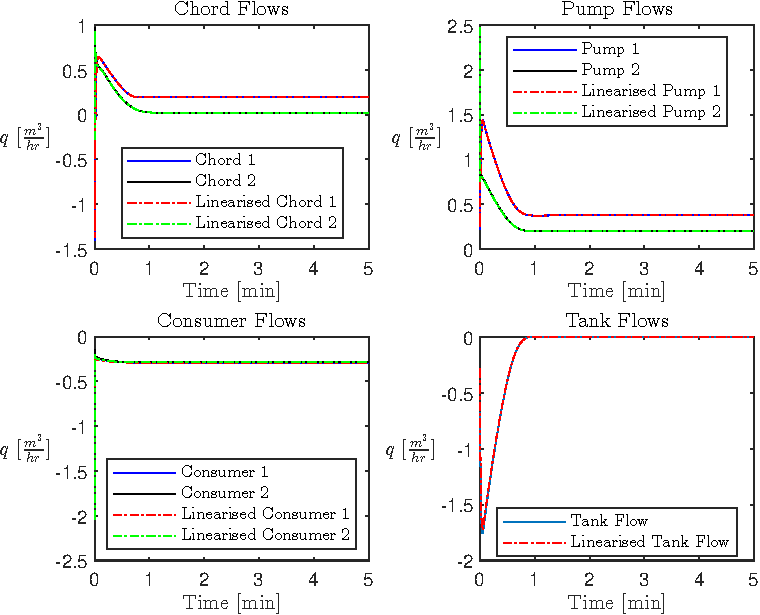
\includegraphics[height = 4cm,width=\linewidth]{Graphics/NominalFlows.pdf}
	\caption{Comparison of non-linear and linearised model behaviour, $1$-step-ahead prediction at operating point}
	\label{fig:CompNonLinEQ}
\end{figure}

Evaluating the model away from the linearisation operating point ($\Theta = \{0.7,0.4\} \wedge \omega = \{80,40\}$), we see per \cref{fig:CompNonLinNotEQ} that the model is still largely accurate.

\begin{figure}[h]
	\centering
	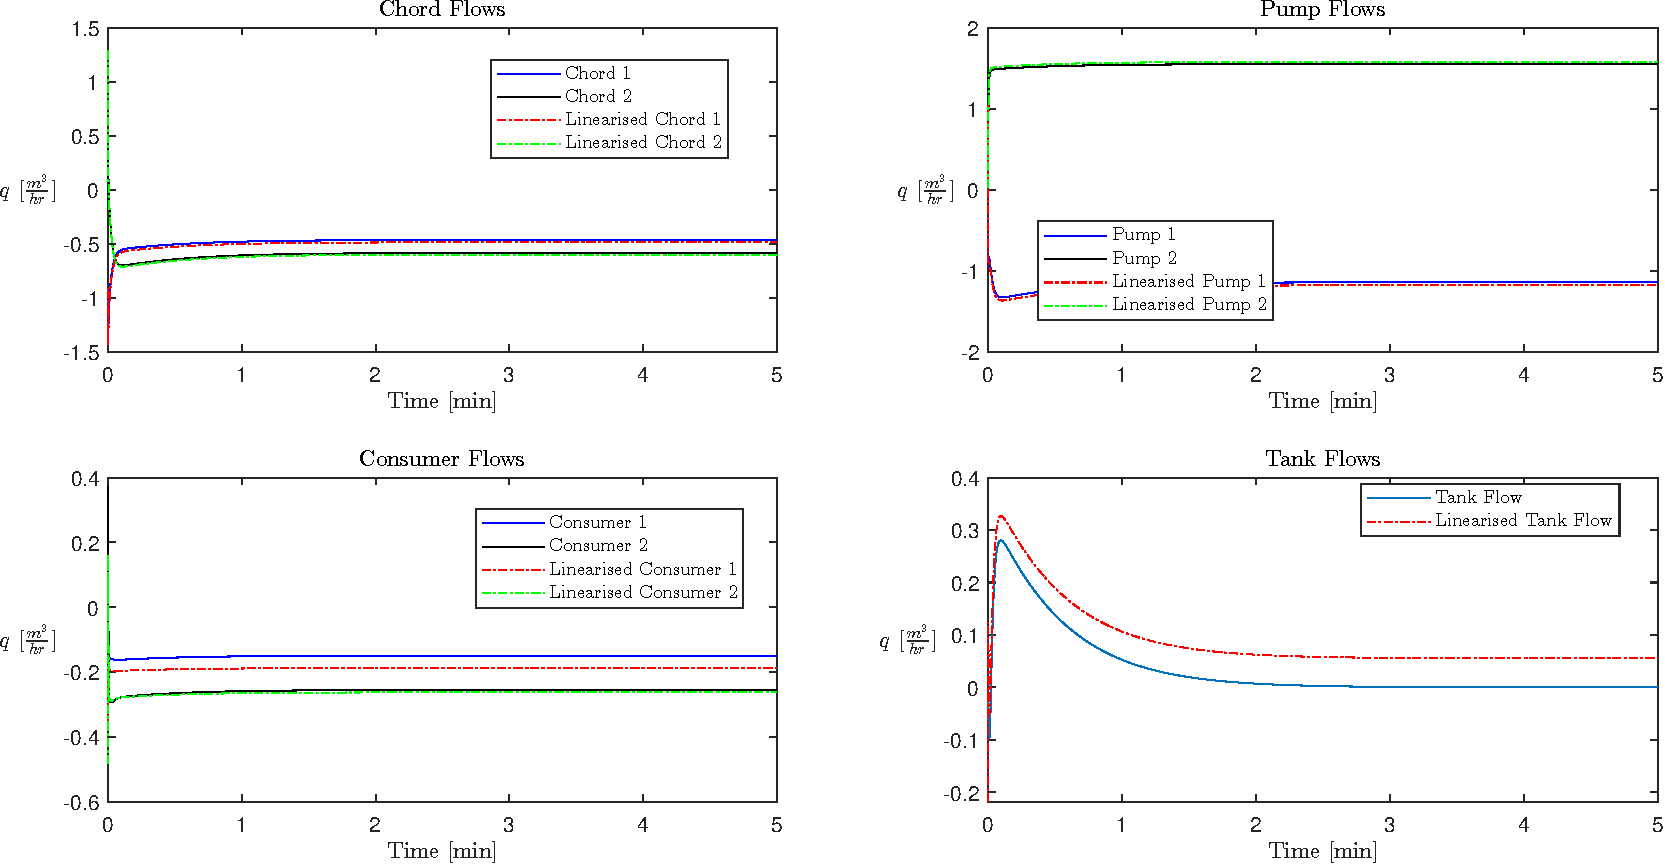
\includegraphics[height=4cm,width=\linewidth]{Graphics/DifferentOPFlows.pdf}
	\caption{Comparison of non-linear and linearised model behaviour, $1$-step-ahead prediction away from operating point}
	\label{fig:CompNonLinNotEQ}
\end{figure}

The largest error is with respect to the chord and consumer flows, which is intuitive as the linearised model assumes a constant valve setting. We note a significant error in the tank flow, but also note that this error is constant as predicted and therefore trivially compensated for with integral action. Having confirmed the small-signal accuracy of the linearised model, we now move on to design of the control algorithm.

\section{Control Structure}\label{sec:ControlStructure}
The control strategy proposed is presented in \cref{fig:tikzControlStrat} and includes the aforementioned inner fast loop and outer slow loop:  

\begin{figure}[h!]
	\centering
	\resizebox{\columnwidth}{!}{
		\begin{tikzpicture}[auto, node distance=2.5cm,>=latex']
	% ========================== Nodes ============================
	% Nodes in upper vertical line
	\node [input, name=rinput] (rinput) {};
	\node [sum, right of=rinput] (sum1) {};
	\node [block, right of=sum1, node distance = 1.5cm] (LQR) {LQR};
	\node [sum, right of=LQR, node distance =
	1.5cm] (sum2) {};
	\node [block, right of=sum2, node distance = 1.5cm] (PID){PID};
	\node [block, right of=PID, align=center] (Fast){Fast\\Dynamics};
	\node [block, right of=Fast, node distance = 3cm, align=center] (Slow){Slow\\Dynamics};
	\node [output, right of=Slow] (output) {};
	
	% Nodes for inner feedback
	\node [tmp, right of=Fast, node distance = 1.5cm] (tmp0){};
	\node [tmp, below of=tmp0, node distance = 1.5cm] (tmp1){};
	\node [tmp, below of=sum2, node distance = 1.5cm] (tmp2){};
	
	% Nodes for outer feedback
	\node [tmp, right of=Slow, node distance = 1.5cm] (tmp10){};
	\node [tmp, below of=tmp10,node distance = 2.5cm] (tmp11){};
	\node [tmp, below of=sum1, node distance = 2.5cm] (tmp12){};
	
	% Nodes for Disturbance
	\node [tmp, above of=tmp0, node distance = 2.5cm] (tmp20){};
	\node [tmp, above of=tmp0, node distance = 2cm] (tmp21){};
	\node [tmp, above of=Fast, node distance = 2cm] (tmp22){};
	\node [tmp, above of=Slow, node distance = 2cm] (tmp23){};
	
	\draw[thick, dotted] ($(Fast.north west)+(-0.25, 0.25)$) rectangle  ($(Slow.south east)+(0.25, -0.25)$);
	\node[above of =tmp0, node distance =1.1cm](sys_txt) {System};
	
	% ========================== Lines ============================
	
	% Lines in upper vertical part of block diagram
	\draw [->] (rinput) -- node{$p_{ref}$} (sum1);
	\draw [->] (sum1) --node[name=z,anchor=north]{} (LQR);
	\draw [->] (LQR) -- node{$ q_{ref} $}(sum2);
	\draw [->] (sum2) -- (PID);
	\draw [->] (PID) -- node[pos=0.4]{$ \omega_{ref} $}(Fast);
	\draw [->] (Fast) -- node{$d_p$}(Slow);
	\draw [->] (Slow) -- node{$p_{\tau}$}(output);	
	
	% Lines for inner feedback
	\draw [-] (tmp0) -- (tmp1);
	\draw [-] (tmp1) -- (tmp2);
	\draw [->] (tmp2) -- node[pos=0.99]{$ - $}(sum2);
	
	
	% Lines for outer feedback
	\draw [-] (tmp10) -- (tmp11);
	\draw [-] (tmp11) -- (tmp12);
	\draw [->] (tmp12) -- node[pos=0.99]{$ - $}(sum1);
	
	
	% Lines for disturbance
	\draw [-] (tmp20)node[above, align=center]{Consumer \\ Disturbance} -- (tmp21);
	\draw [-] (tmp21) -- (tmp22);
	\draw [-] (tmp21) -- (tmp23);
	\draw [->] (tmp22) -- node[left, pos = 0.5]{$\Theta$}(Fast);
	\draw [->] (tmp23) -- node[pos = 0.5]{$ d_c $}(Slow);
	
	
\end{tikzpicture}
}
	\caption{Control Strategy including control for fast and slow dynamics}
	\label{fig:tikzControlStrat}
\end{figure}

We will first address the outer LQR controller. This is an optimal controller that, in its general form, is given by the solution to the Lagrange problem:

\begin{equation}\label{eq:LagrangeProblem}
		J = \int_{t_0}^{\infty} \big(x^T(t)Qx(t) + u^T(t)Ru(t)\big)dt
\end{equation} 

constrained by the dynamics:

\begin{equation}\label{eq:LQRDynamicsConstraint}
	\begin{gathered}
		\dot{x}(t) = Ax(t) + Bu(t) \\
		x(t_0) = x_0
	\end{gathered} 
\end{equation}

The optimal solution to this problem is given by minimising the Hamiltonian $\mathcal{H}$ \cite{Liberzon2012}:

\begin{equation}\label{eq:Hamiltonian}
	\begin{gathered}
			\mathcal{H} = \lambda^T(t) f(x(t),u(t)) - \mathcal{L}(x(t),u(t)) \\
			f(x(t),u(t)) = A(t)x(t) + B(t)u(t) \\
			\mathcal{L}(x(t),u(t)) =  x^T(t)Q(t)x(t) - u^T(t)R(t)u(t)
	\end{gathered}
\end{equation}

which gives a solution of the type:

\begin{equation}\label{eq:LQRSolution}
	u^*(t) = -RB^TPx^*(t) = -Kx^*(t)
\end{equation}

where $P$ is the solution to the algebraic Riccatti equation:

\begin{equation}\label{eq:ARE}
	PA + A^TP + Q - PBR^{-1}B^TP = 0
\end{equation}

However, the standard LQR has several major issues. It only regulates to the origin, it does not have integral action, and it does not reject state disturbances. We therefore, as in Pannocchia et al. \cite{Pannocchia2015a} rewrite the above as a discrete problem in deviation variables and solve:

\begin{equation}\label{eq:LagrangeProblemDeviation}
	\begin{gathered}
	J = \sum_{k_0}^{\infty} \big(\zeta(k)^TQ\zeta(k) + \tilde{u}(k)^TR\tilde{u}(k)\big) \\
	\zeta = \begin{bmatrix}	x(k)-x(k-1) \\ y(k)-r(k) \end{bmatrix}, \quad \tilde{u}(k) = u(k)-u(k-1) 
	\end{gathered}
\end{equation} 

where the constraining dynamics are given by:

\begin{equation}\label{eq:VelocityMatrices}
	\begin{gathered}
		\zeta(k+1) = \tilde{A}\zeta(k) + \tilde{B}\tilde{u}(k) \\
		\tilde{A} = \begin{bmatrix} A & 0 \\ CA & I	\end{bmatrix}, \ 
		\tilde{B} = \begin{bmatrix} B \\ CB	\end{bmatrix}, \ \tilde{C} = \begin{bmatrix} 0 & I	\end{bmatrix}
	\end{gathered}
\end{equation}

and the optimal control policy becomes:

\begin{equation}\label{eq:OptimalVFLQRPolicy}
\begin{gathered}
\tilde{u}^*(k) = -\tilde{K}\tilde{x}^*(k) \\
u^*(k) = \sum_{i=1}^{k} \tilde{u}^*(k)
\end{gathered}
\end{equation}

This control policy, however, still lacks disturbance rejection. Assuming that we are only concerned with optimal control of the disturbance-free subsystem, complete rejection of the state disturbance $\delta(k)$ can then be achieved by augmenting \cref{eq:OptimalVFLQRPolicy} \cite{Singh2017}:

\begin{equation}
	u(k) = \sum_{i=1}^{k} \tilde{u}^*(k) - B^\dagger B\delta(k)
\end{equation}

where $B^\dagger$ is the Moore-Penrose pseudoinverse of $B$.

%\begin{equation}\label{eq:InfLQRHamiltonian}
%	\mathcal{H}(x(t),u(t),\lambda(t),t)) = \lambda^T(t)\big(Ax(t) + Bu(t)\big) - x^T(t)Qx(t) - u^T(t)Ru(t)
%\end{equation}








\section{Results}\label{sec:Results}
The viability of the proposed control structure is validated in the Aalborg University Smart Water Infrastructure Laboratory (SWIL). This modular laboratory consists of a number of units pumping units (PU), consumer units (CU), and piping units (PiU) that can be used for small-scale emulation of a real WDN.

\begin{figure}[h!]
	\includegraphics[height=4cm, width=\linewidth]{Graphics/SWIL.pdf}
	\caption{Picture of the AAU SWIL}
	\label{fig:AAUSWIL}
\end{figure}

The network topology in \cref{fig:WDNModel} is emulated via two PUs, a CU with two adjustable one-way valves each emulating a consumer, and a CU with an open bidirectional valve acting as the EWR, interconnected via two PiUs. Geodesic heights are emulated by pressurising the CUs. Experiments run for $12$ hours, with consumer demand curves based on real data and compressed to a fundamental frequency of $4$ hours such that each experiment corresponds to $3$ days. The controller attempts to follow a constant level reference throughout, starting $15 \si{mm}$ beneath it. After $4$ hours, a system leakage is simulated by fully opening the consumer valves for $30$ seconds. After $8$ hours, $50\%$ packet loss is introduced in the outer loop, which operates on a simulated TOD protocol. The tank level is seen on \cref{fig:OuterLoop}, while a snapshot of pump behaviour is seen on \cref{fig:InnerLoop}. The disturbance estimation scheme and true consumer flows can be seen on \cref{fig:DisturbanceEstimation}, with a zoomed-in view around the leakage seen on \cref{fig:Leakage}.

%We first present results pertaining to the VF-LQR. The controller is tested against nominal conditions, a variety of non-nominal time constants, and against a constant output disturbance. In each case the controls are clamped corresponding to the provided pump curves \cite{GrundfosDatablad}, the system is subjected to a varying state disturbance, and a sampling time of $t_s = 10\si{min}$ is assumed. The results can be seen on \cref{fig:LQRTracking}, displaying good tracking performance in each case; the disturbance is completely rejected, and the system tracks the reference. In all cases $Q = \left(\tilde{C}^T\tilde{C}\right)$ and $R = \text{diag}(0.1)$; the former guarantees an exponentially stable closed-loop system \cite{Liberzon2012}.


\begin{figure}[h!]
	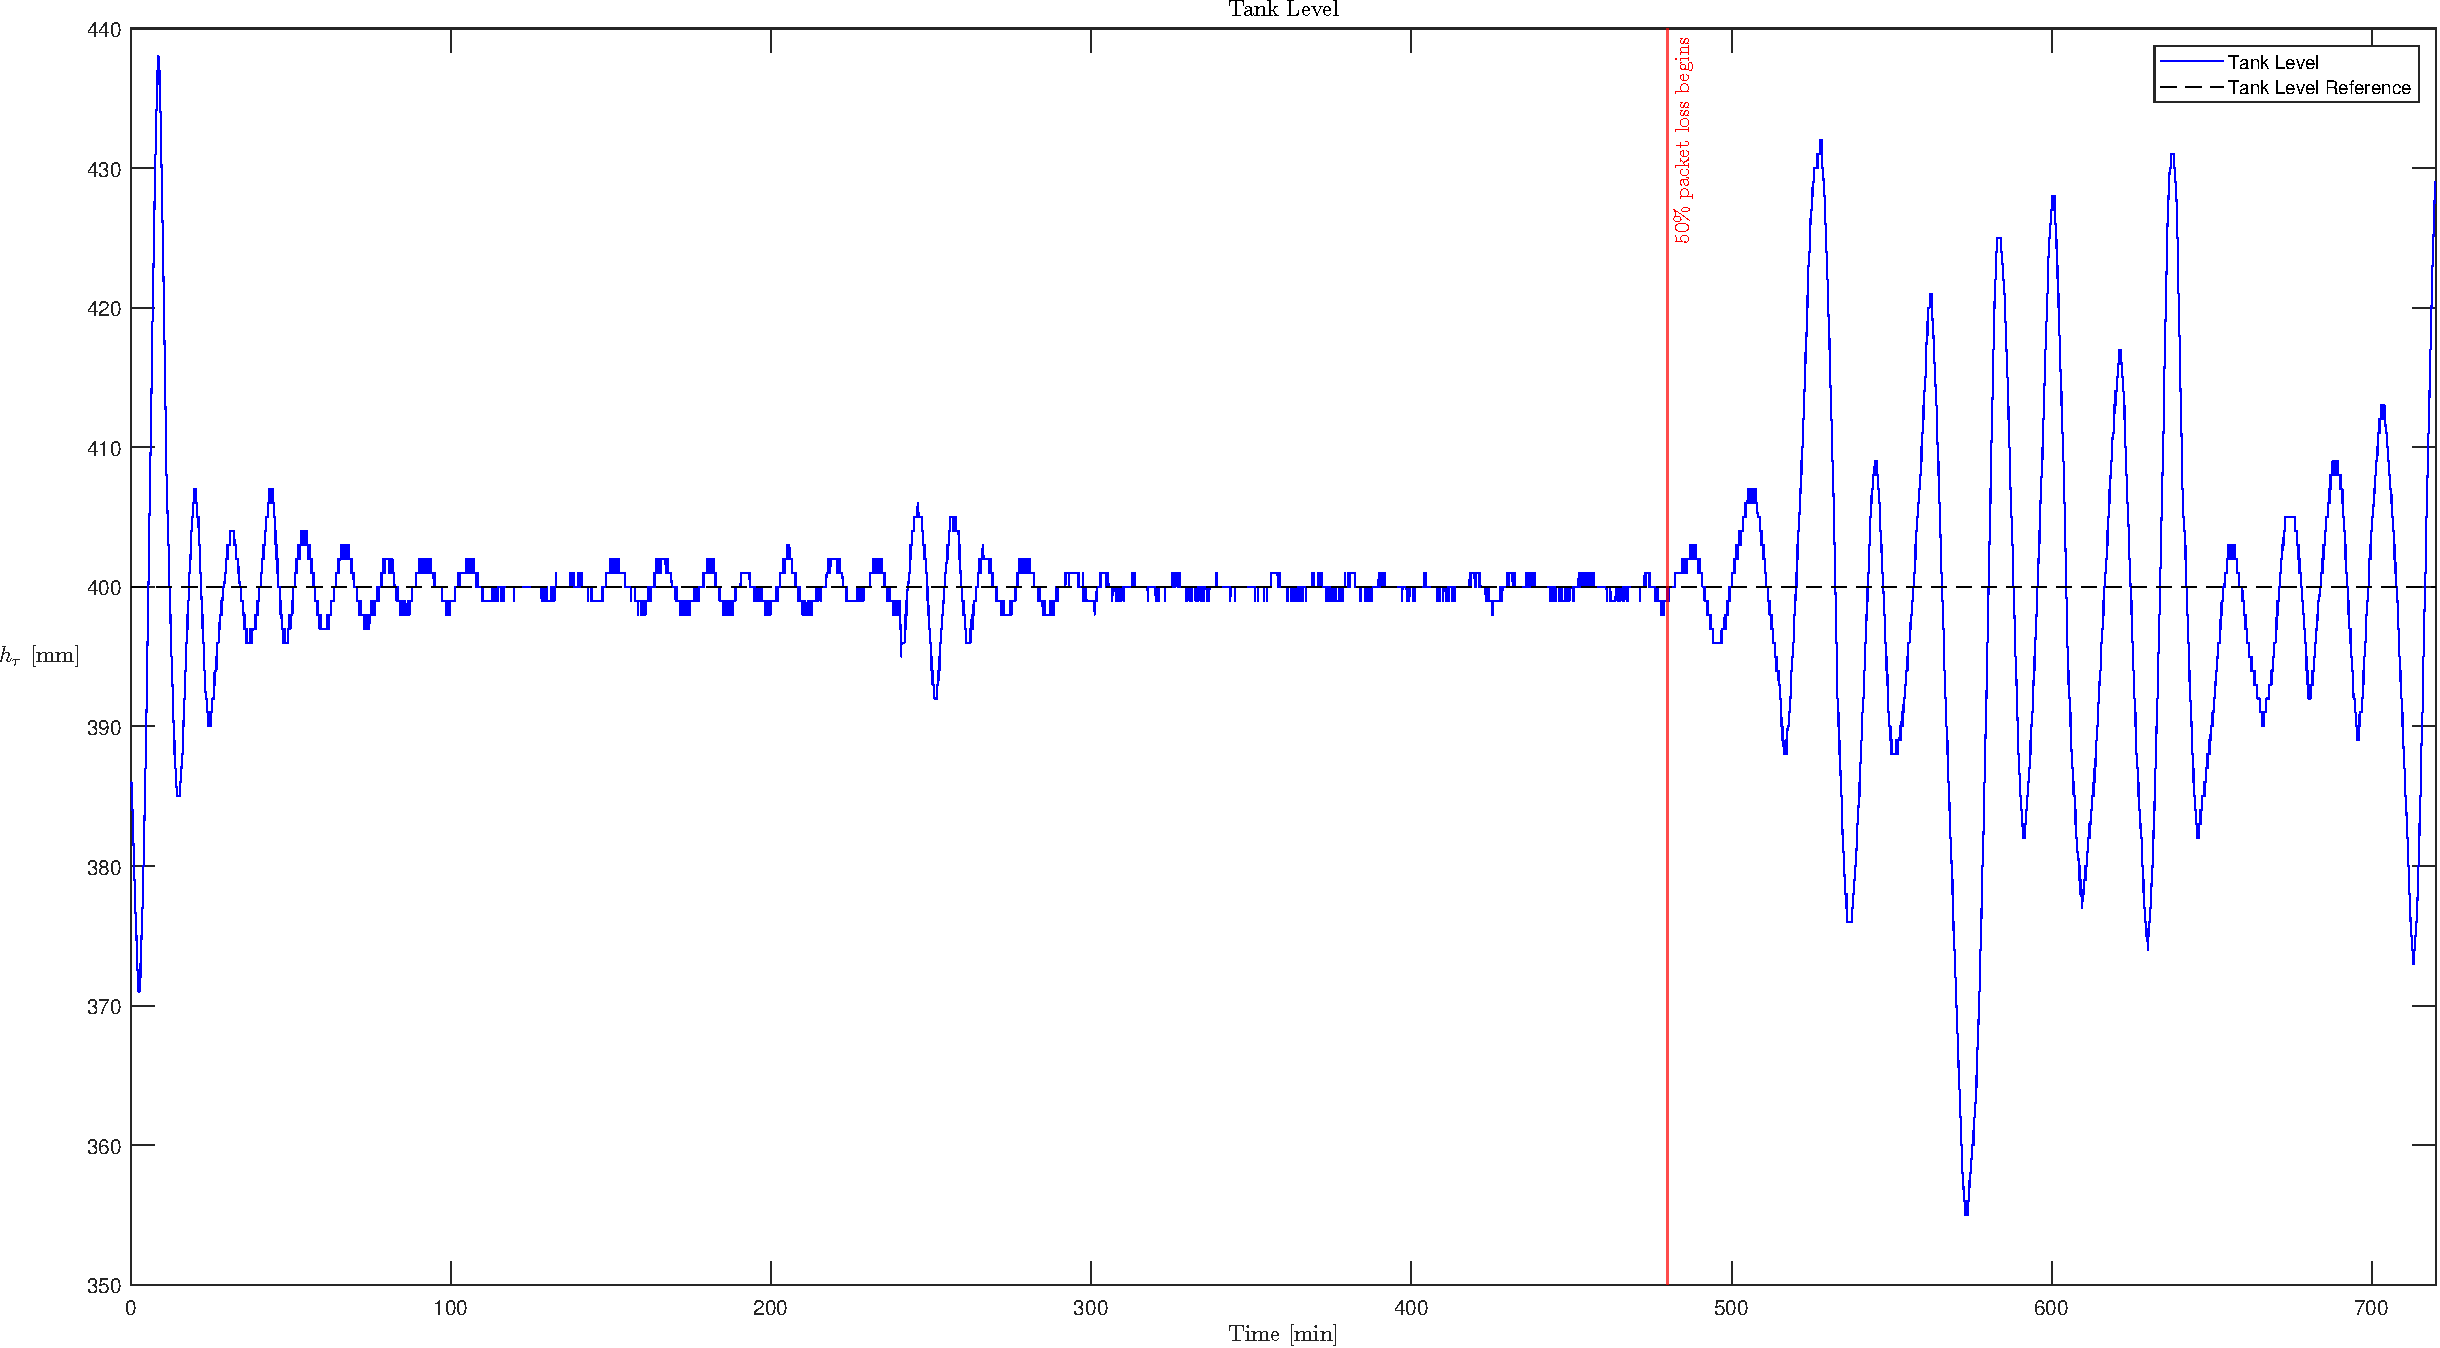
\includegraphics[height=4cm, width=\linewidth]{Graphics/OuterLoop.pdf}
	\caption{Outer loop.}
	\label{fig:OuterLoop}
\end{figure}


\begin{figure}[h!]
	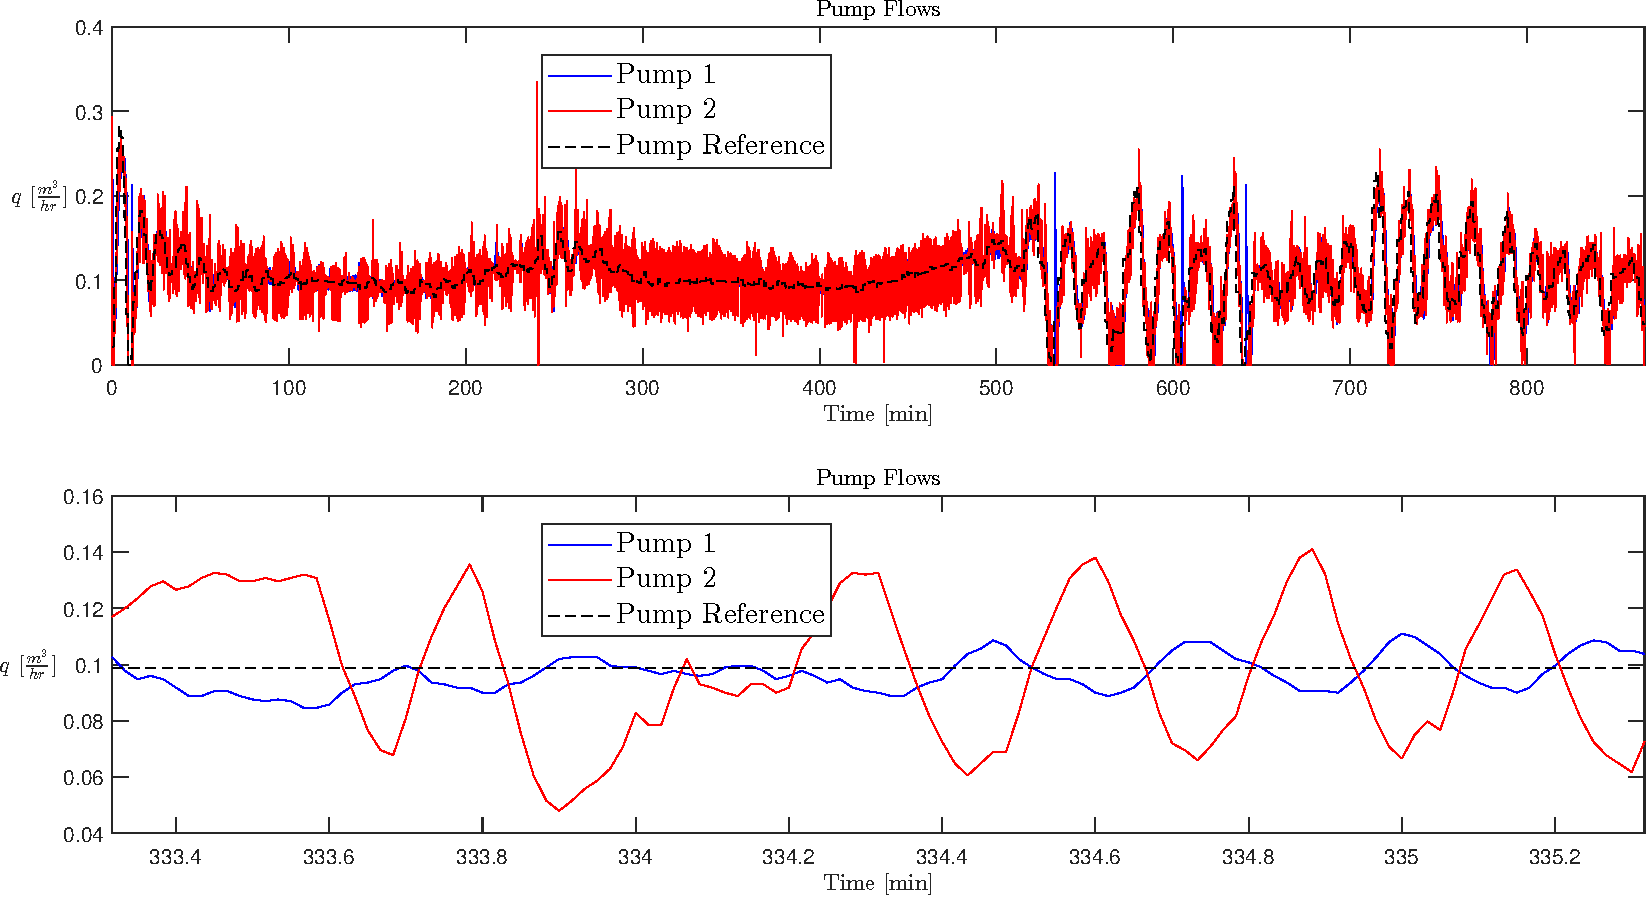
\includegraphics[width=\linewidth,height=4cm]{Graphics/InnerLoop.pdf}
	\caption{Inner loop.}
	\label{fig:InnerLoop}
\end{figure}


\begin{figure}[h!]
	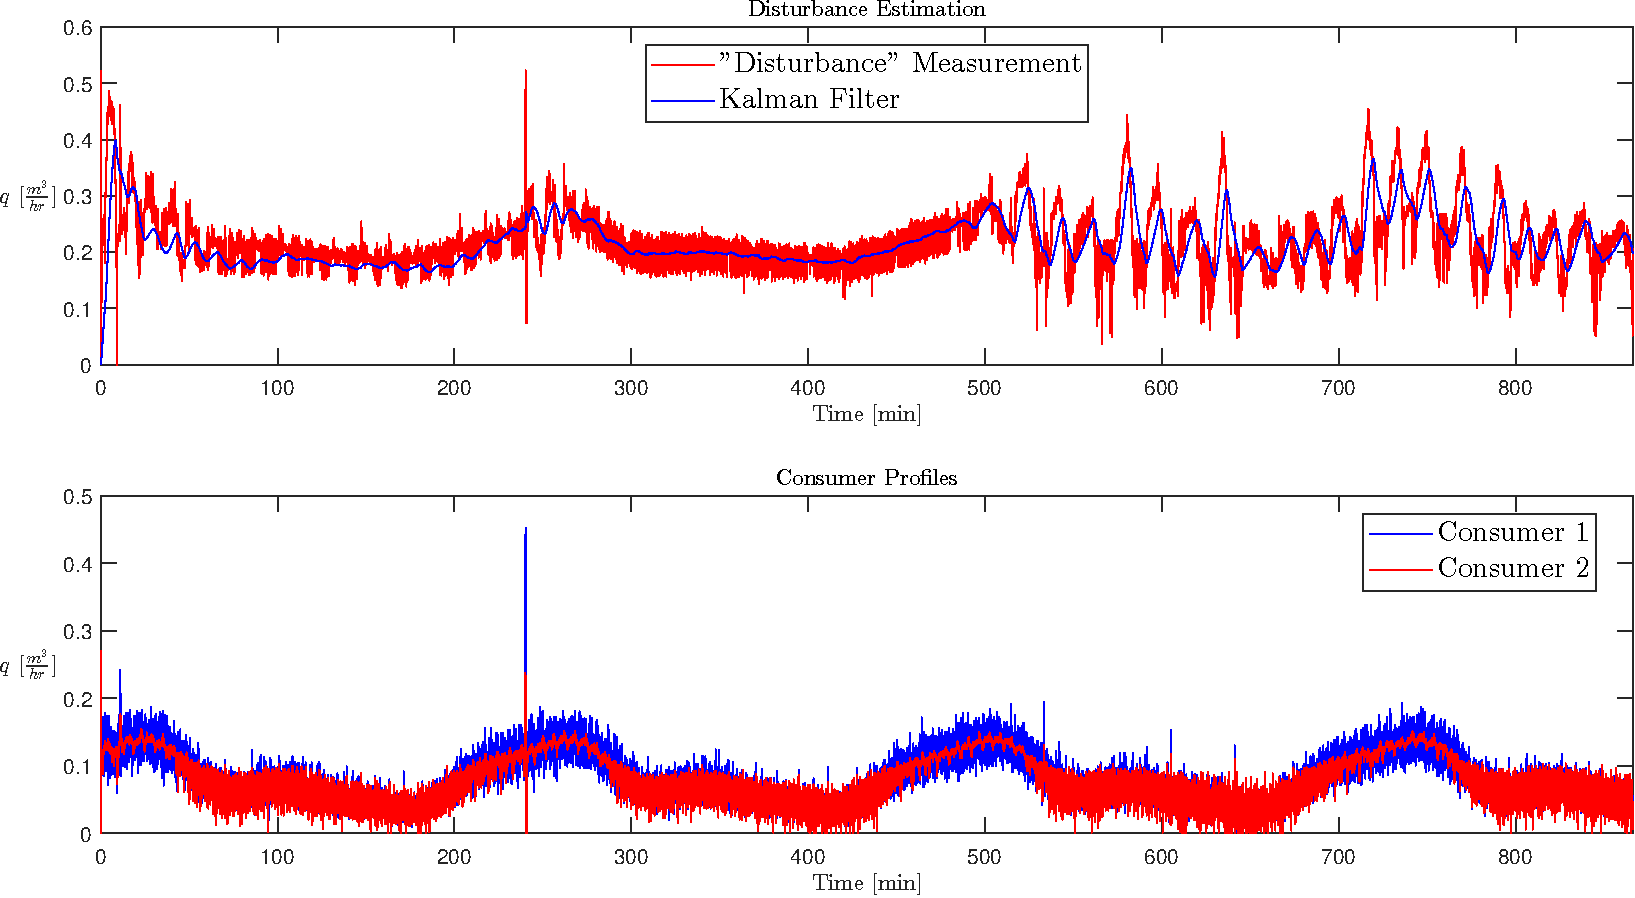
\includegraphics[height=4cm, width=\linewidth]{Graphics/DisturbanceEstimation.pdf}
	\caption{Consumer disturbance estimation.}
	\label{fig:DisturbanceEstimation}
\end{figure}

\begin{figure}[h!]
	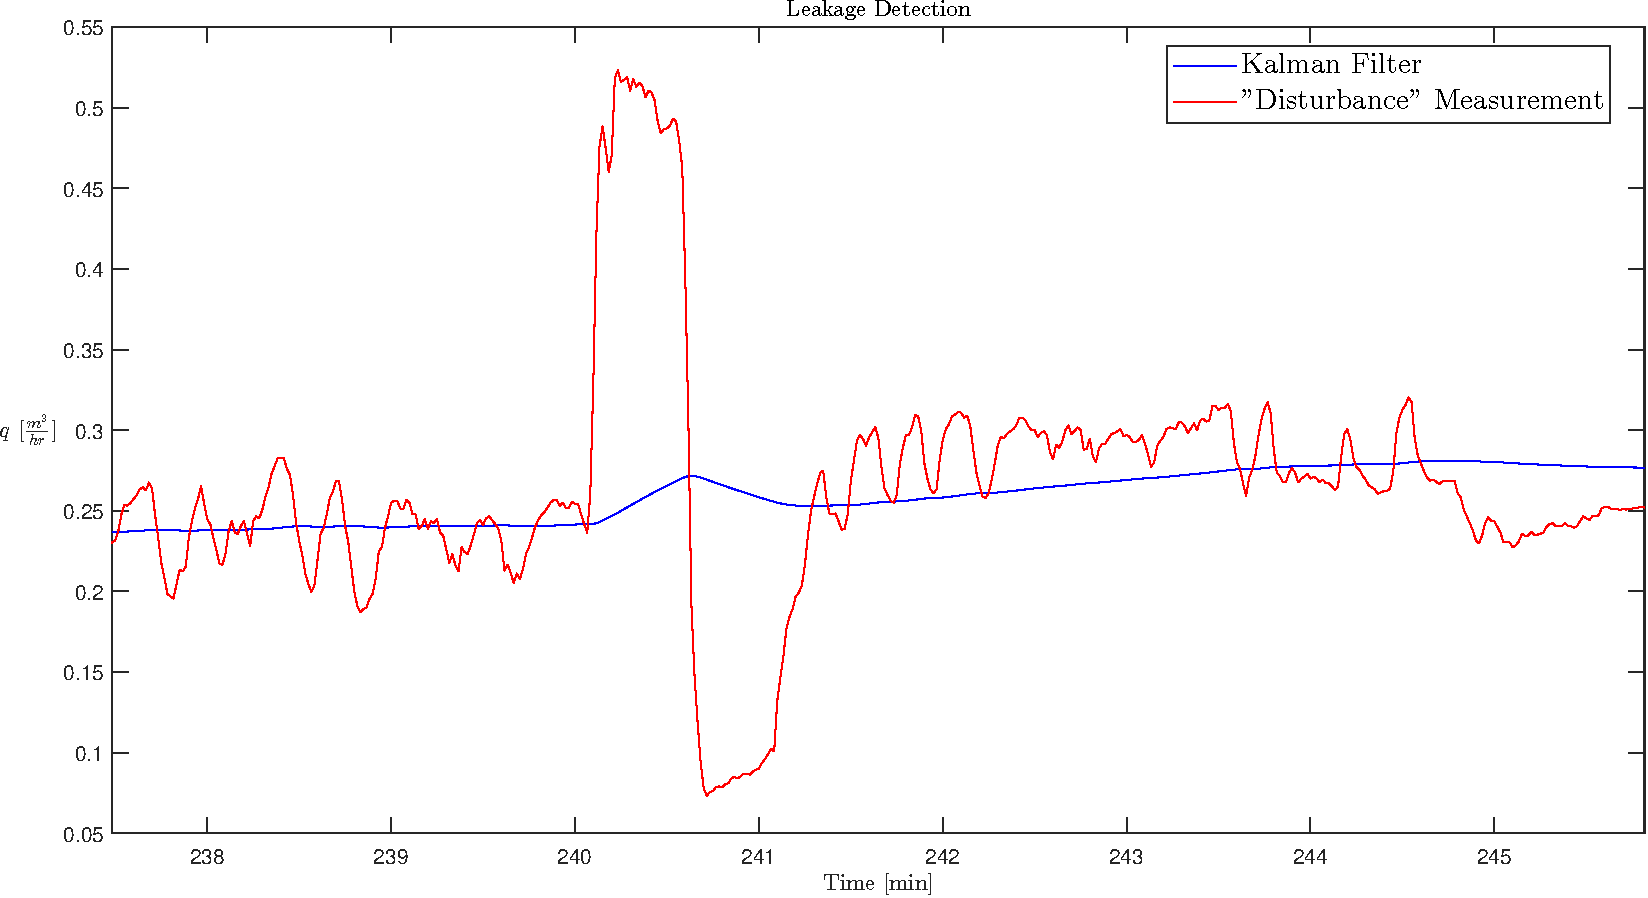
\includegraphics[height=4cm, width=\linewidth]{Graphics/LeakageDetection.pdf}
	\caption{Leakage detection.}
	\label{fig:Leakage}
\end{figure}





\newpage
\section{Conclusion}\label{sec:Conclusion}
Again we conclude that we have done everything correct and that we are completely awesome.

% conference papers do not normally have an appendix


% use section* for acknowledgment
\section*{Acknowledgment}
The authors would like to thank our advisors Saruch Satishkumar Rathore and carsten skovmose kallesøe beyond what could be expected. 









% trigger a \newpage just before the given reference
% number - used to balance the columns on the last page
% adjust value as needed - may need to be readjusted if
% the document is modified later
%\IEEEtriggeratref{8}
% The "triggered" command can be changed if desired:
%\IEEEtriggercmd{\enlargethispage{-5in}}

% references section

% can use a bibliography generated by BibTeX as a .bbl file
% BibTeX documentation can be easily obtained at:
% http://mirror.ctan.org/biblio/bibtex/contrib/doc/
% The IEEEtran BibTeX style support page is at:
% http://www.michaelshell.org/tex/ieeetran/bibtex/
%\bibliographystyle{IEEEtran}
% argument is your BibTeX string definitions and bibliography database(s)
%\bibliography{IEEEabrv,../bib/paper}
%
% <OR> manually copy in the resultant .bbl file
% set second argument of \begin to the number of references
% (used to reserve space for the reference number labels box)

\bibliographystyle{ieeetran}
\bibliography{../../RefLib/CA7Projekt.bib}



% that's all folks
\end{document}


